\chapter{Relevamiento de aplicaciones de \emph{video mapping}}
\section{\emph{Modul8}}
\emph{Modul8}\cite{Module8} es una herramienta profesional diseñada para realizar espectáculos de proyección de video en vivo diseñada por \emph{VJs} y se encuentra disponible exclusivamente para plataforma \emph{Mac OS} mediante licenciamiento propietario.

\begin{figure}[H]
  \centering
    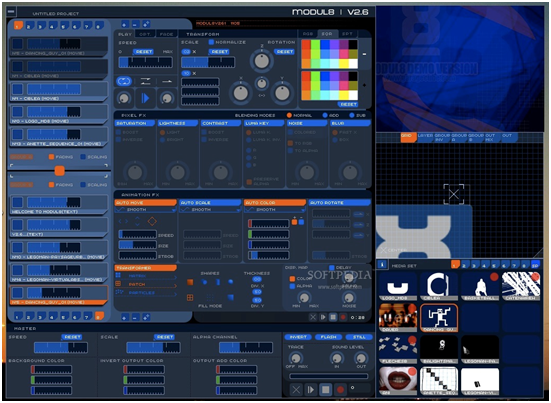
\includegraphics[width=0.6\textwidth]{./Cap3_aplicaciones/apps-modul8.png}
  \caption{Pantalla principal de \emph{Modul8}}
  \label{fig:Apps-Module8}
\end{figure}

La interfaz de usuario está pensada para los espectáculos en vivo, para lo que cuenta con cuatro paneles con funcionalidad bien específica: un panel principal donde crear y editar las composiciones de video, sonido y efectos; un panel multimedia para administrar los archivos de medios (videos, imágenes, pistas de audio, etc.); un panel de previsualización donde se puede ir observando la ejecución de una parte de la composición del espectáculo; y por último el panel de salida, donde se observa la composición final que será proyectada. Todas las funcionalidades provistas pueden ser asignadas a eventos \emph{MIDI}\footnote{MIDI}, por lo que es posible utilizar cualquier dispositivo que los genere para controlar enteramente la aplicación.
\emph{Modul8} maneja hasta siete salidas simultáneas de proyección y una más para la interfaz de usuario. Para hacer uso de esta funcionalidad es necesario contar con una tarjeta de video que dé soporte a la salida múltiple. Esto activa el modo de salida avanzado dando se puede escoger entre varias alternativas para la selección de la composición o porción de la misma a ser emitida en cada una de las salidas disponibles. \emph{Modul8} maneja el concepto de capa, con un máximo de diez, las cuales pueden contener sus propios medios, efectos y configuraciones.
Si bien no hay un manejo tridimensional de la escena, la aplicación provee algunas transformaciones a aplicar a los medios para ajustarlos a la representación bidimensional de los objetos de la escena o incluso a objetos tridimensionales autogenerados que aparecerán en la misma.
La arquitectura de la herramienta permite su extensión mediante la programación de módulos o efectos en el lenguaje \emph{Python}\footnote{\emph{Python}}.
En cuanto al rendimiento, se hace un uso intensivo de la unidad de procesamiento gráfica o \emph{GPU}\footnote{Ver glosario.} para todo lo que es dibujado, composición y transformaciones de gráficos.

\section{\emph{VDMX}}
\emph{VDMX}\cite{VDMX} es una aplicación para el procesamiento multimedia en tiempo real, disponible exclusivamente para plataforma \emph{Mac OS} mediante licenciamiento propietario. Su arquitectura modular la hace altamente personalizable.

\begin{figure}[H]
  \centering
    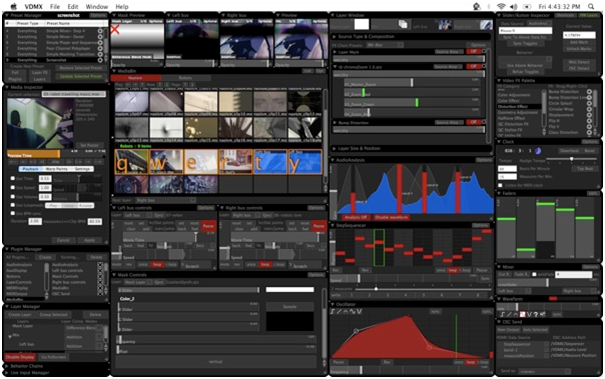
\includegraphics[width=0.6\textwidth]{./Cap3_aplicaciones/apps-vdmx.png}
  \caption{Ejemplo de consola personalizable avanzada realizada en VDMX}
  \label{fig:Apps-VDMX}
\end{figure}

Para ello provee funcionalidad básica mediante lo que la aplicación denomina inspectores. El inspector del grupo de trabajo expone todo lo que esta sucediendo en \emph{VDMX} a bajo nivel, como ser los archivos multimedia, las entradas de video configuradas, las capas, los \emph{plugins} existentes, etc. Luego, el inspector de interfaz de usuario permite ver y editar las propiedades de cada control que se selecciona en la interfaz. Adicionalmente, permite crear interfaces propias a partir de controles básicos como deslizadores, botones, ventanas emergentes, etc, lo que permite a los \emph{VJs} tener toda la información que crea relevante a disposición en el momento de la representación en vivo.
La aplicación permite asociar eventos de entrada \emph{MIDI}, \emph{OSC} o de teclado a cualquier control de la interfaz de usuario, así como también generar eventos \emph{MIDI} u \emph{OSC} para ser consumidos por cualquier aplicación externa que los soporte.
Las capas contienen una única fuente de medios, la que puede ser de tipo video, composición de \emph{QuartzComposer}\footnote{QuartzComposer} o imagen, y adicionalmente se define una cadena de efectos a ser aplicados a la fuente de la capa. La ejecución de la secuencia de efectos puede ser configurada mediante cualquiera de los mecanismos de eventos mencionados anteriormente así como por tiempo. No hay un máximo establecido en el número de capas que se pueden crear en \emph{VDMX}, y es posible agruparlas para darle un manejo diferenciado o aplicar efectos a todas a la vez.
Se cuenta con tres modos de salida de video: ventana, pantalla completa y avanzado. En el modo avanzado se permite crear dispositivos de salida, sin un limite predeterminado, y asociarlos a las capas o dispositivos de entrada que se desee.

\section{\emph{VVVV}}
\emph{VVVV}\cite{VVVV} es una herramienta de programación de propósito general que provee un entorno híbrido de programación gráfica y textual. Es de uso gratuito para propósitos no comerciales y se encuentra disponible únicamente para plataformas Windows.

\begin{figure}[H]
  \centering
    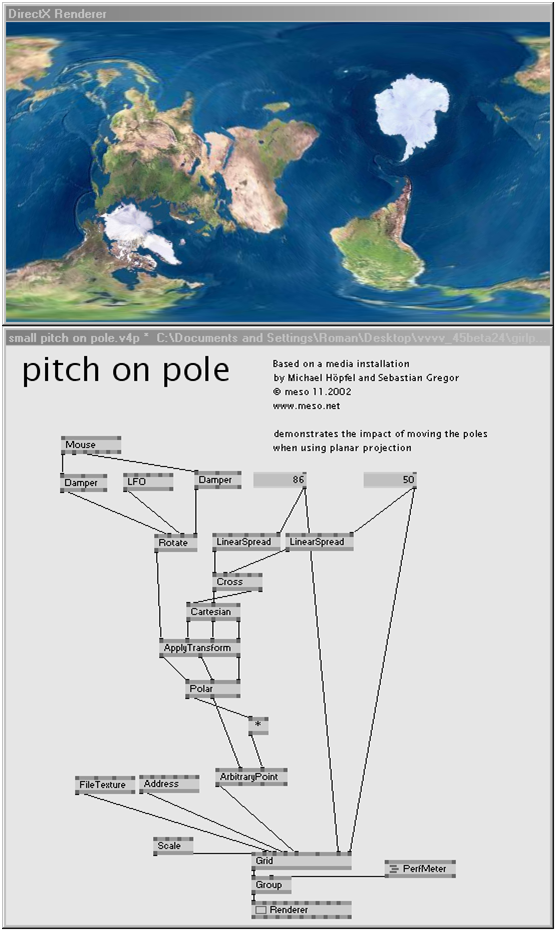
\includegraphics[width=0.5\textwidth]{./Cap3_aplicaciones/apps-vvvv.png}
  \caption{Entorno de programación de \emph{VVVV} y salida de video correspondiente}
  \label{fig:Apps-VVVV}
\end{figure}

Para la construcción de un programa se utilizan nodos que representan operaciones o funciones individuales que pueden, eventualmente, tomar una entrada, procesarla, y entregar datos a la salida. Las conexiones entre nodos se llaman \emph{links} y es como se modela el flujo de información entre nodos.
Existen varios tipos de nodos para diferentes propósitos. A modo de ejemplo, el nodo utilizado para desplegar la salida visual del programa es del tipo \emph{renderer}, para el agregado de cuadrantes se utiliza el nodo \emph{quad}, para el manejo de transformaciones el nodo \emph{transform} y para redimensionar a escala el nodo \emph{scale}. También hay nodos para cargar objetos tridimensionales, manejar texturas, vectores, temporizadores, etc. Todo en \emph{VVVV} es representado a través de nodos.
A diferencia de otros lenguajes de programación, los que cuentan con diferentes modos para construir y ejecutar los programas, \emph{VVVV} todo el tiempo trabaja en un solo modo, el modo de ejecución. En él, constantemente se están ejecutando cálculos y dibujando gráficos mientras se está generando o editando un programa.
Para dar soporte multiproyector, \emph{VVVV} implementa una arquitectura cliente-servidor, la que permite contar con cualquier cantidad de motores tridimensionales (clientes) manejados desde una instancia de VVVV central (servidor). Toda la configuración y ejecución de un espectáculo distribuído se implementa en un módulo llamado \emph{boygrouping}\footnote{http://vvvv.org/documentation/boygrouping-basics}.
\emph{VVVV} provee soporte para varios protocolos de entrada y salida como \emph{TCP}, \emph{UDP}, \emph{MIDI} y \emph{OSC} entre otros, y gracias a aportes de la comunidad de programadores \emph{VVVV} es posible también interactuar con dispositivos como \emph{Wii}, \emph{PSP} y \emph{Kinect}. Existen nodos que proveen funcionalidad avanzada como ser soporte para animación y líneas de tiempo, detección y seguimiento de objetos en tiempo real utilizando variadas técnicas como \emph{ARToolkit} y \emph{OpenCV} entre otras, emisión de flujos de video, reproducción y mezcla de archivos de audio, simulación de movimiento, colisiones y efectos físicos en general.
El motor gráfico tridimensional de \emph{VVVV} está basado en \emph{Direct3D}\footnote{Direct3D}, lo que permite hacer un uso intensivo de las placas gráficas modernas para el dibujado de gráficos de alto rendimiento.
\emph{VVVV} ofrece la posibilidad de crear nodos personalizados a través de una interfaz \emph{COM} para la implementación de \emph{plugins}, lo que ofrece varias alternativas en cuanto a la implementación, pudiéndose utilizar \emph{C\#}, \emph{Delphi} o incluso \emph{C++}.

\section{\emph{VPT - Video Projection Tool}}
\emph{VPT}\cite{VPT} es una herramienta para la realización de proyecciones en tiempo real. Es una aplicación de código abierto y de uso y distribución gratuito mediante licenciamiento GNU GPL\footnote{GNU GPL}. Se encuentra disponible para plataformas Windows y MacOS.

\begin{figure}[H]
  \centering
    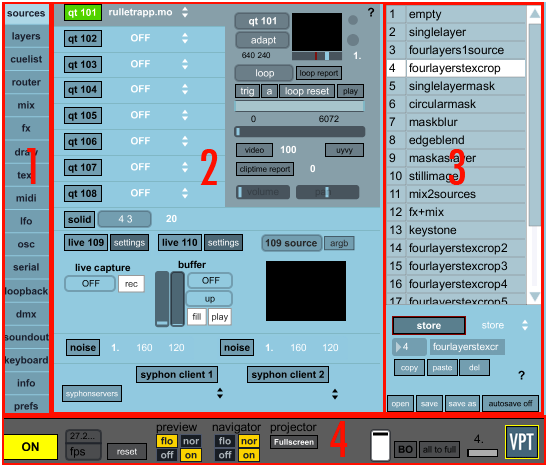
\includegraphics[width=0.65\textwidth]{./Cap3_aplicaciones/apps-vpt.png}
  \caption{Pantalla principal de \emph{VPT}}
  \label{fig:Apps-VPT}
\end{figure}

La interfaz gráfica es amplia y permite el acceso a variadas funcionalidades. Se tiene una barra de herramientas con cada una de las secciones disponibles, las que se muestran en detalle en el panel principal de la aplicación. Siempre disponible a la derecha, están las configuraciones establecidas y predefinidas. La barra sobre el borde inferior de la pantalla es desde donde se controlan las salidas de video, la previsualización y las opciones de navegación.
En cuanto a los posibles orígenes de medios, se puede contar con hasta ocho videos de \emph{quicktime}, dos entradas en vivo, las que pueden ser asociadas a cualquier dispositivo de video soportado en el sistema, y una entrada de dibujado en la que es posible crear máscaras personalizadas para objetos sobre los cuales se proyectará.
Hay una cantidad máxima de 32 capas que se pueden utilizar simultáneamente en un espectáculo. Cada una está superpuesta sobre la siguiente, y puede ser escalada, posicionada, rotada, distorsionada y enmascarada de manera independiente. También es posible asociar fuentes multimedia. Se maneja el concepto de "capa activa" para la edición y dibujado en la ventana de salida.
Se cuenta con una secuencia de eventos a partir de efectos predefinidos almacenados y configurados previamente en el sistema. Para la definición de efectos se cuenta con tipos predefinidos y una nomenclatura para agregarlos a la lista también definida, por ejemplo "F 15 16 5.00" representa una transición del efecto 15 al 16 con duración 5 segundos, "C 5" ejecuta el efecto número cinco, "L 3" genera un bucle y vuelve al tercer lugar de la lista de eventos, "D 2" genera una demora de dos segundos y continúa con el siguiente evento, etc.

\begin{figure}[H]
  \centering
    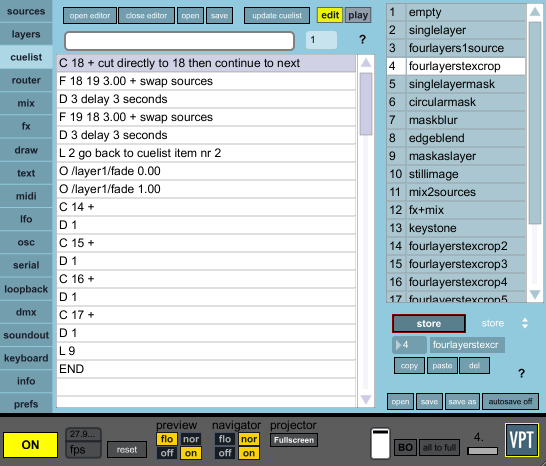
\includegraphics[width=0.65\textwidth]{./Cap3_aplicaciones/apps-vpt-cuelist.png}
  \caption{Efectos y secuencia de eventos de un espectaculo realizado en VPT}
  \label{fig:Apps-VPTCuelist}
\end{figure}

Dentro del modo de edición es posible agregar o eliminar elementos a la lista sin que estos sean reflejados en la salida de video, mientras que en modo de reproducción se está recorriendo la lista de efectos constantemente, generando la salida correspondiente.
Dependiendo de la tarjeta de sonido con la que se cuente, es posible direccionar las entradas de video en hasta ocho canales de salida de audio. El módulo de mezclado permite combinar dos orígenes cualesquiera utilizando diferentes modos. También es posible controlar la aplicación o enviar directamente indicaciones a las capas, orígenes de medios, mezclador, etc, utilizando \emph{OSC}, \emph{MIDI} o vía puerto serial con dispositivos como \emph{arduino}\footnote{http://www.arduino.cc}.
Para simular proyecciones tridimensionales se cuenta con la posibilidad de subdividir las texturas con mallas y aplicar así distorsiones a una capa dada.
%Ver aquí un ejemplo de mallas combinado con el uso de MacOS Syphon Recorder (Syphon MacOS Plugin http://syphon.v002.info/). (http://hcgilje.wordpress.com/2011/05/26/vpt-5-5-preview/)
